\begin{figure}[H]
	\centering
    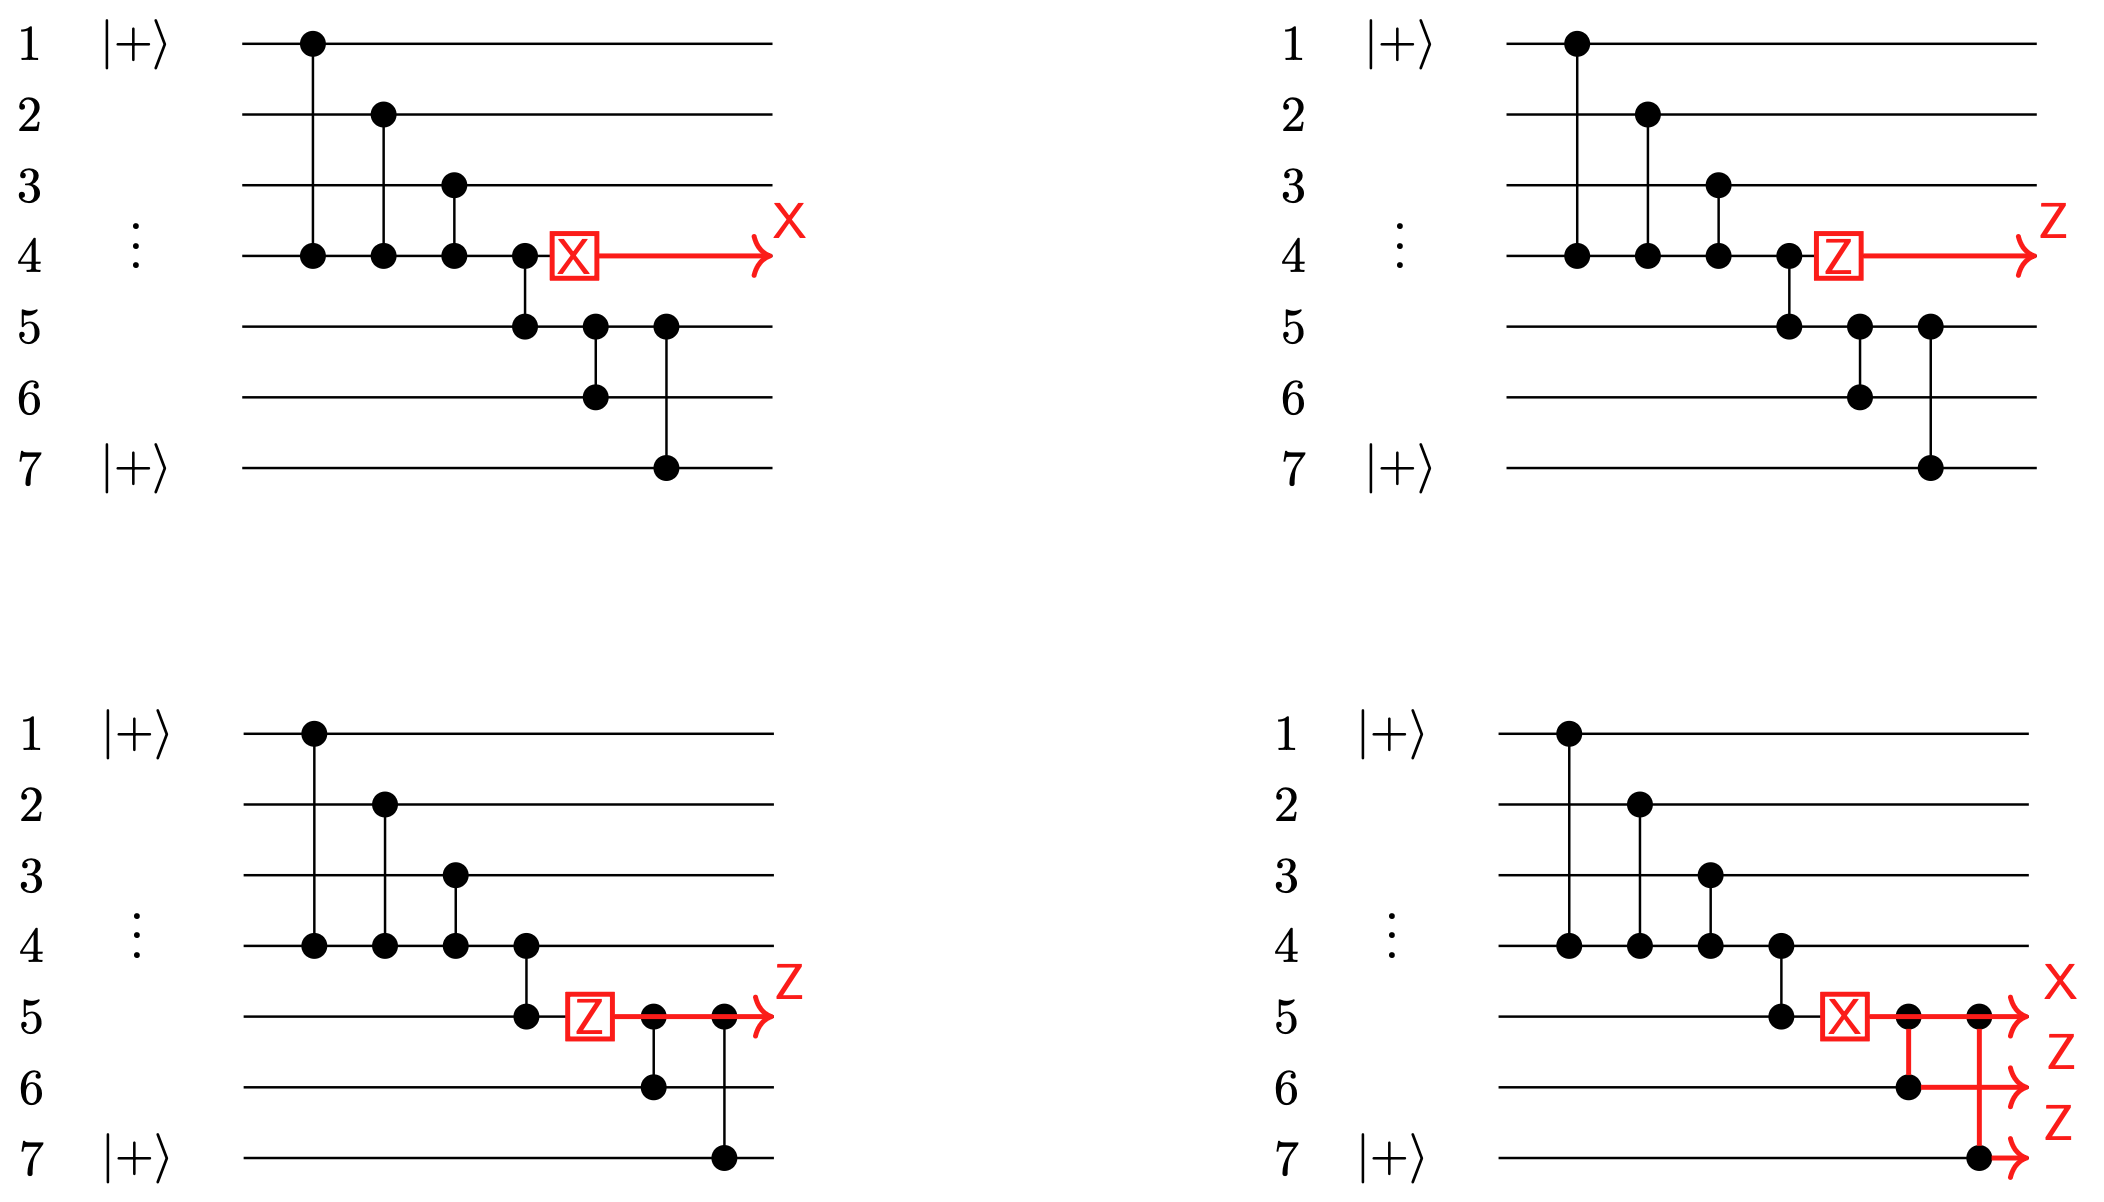
\includegraphics[scale=0.32]{propa.png}
\caption{Propagation of Pauli errors after the faulty $\CZ_{(4,5)}$ gate. The red boxed Pauli operator indicates the error immediately after the faulty gate, and each panel shows its propagation through the remaining $\CZ$ gates in the circuit. A $\X$ error on qubit $4$ (Top left). A $\Z$ error on qubit $4$ which remains localized on $4$ (Top right). A $\Z$ error on qubit $5$ which remains localized on $5$ (Bottom left). An $\X$ error on qubit $5$, which propagates forward through subsequent $\CZ$ gates,
	leaving $\Z$ errors on later neighboring qubits $6$ and $7$ while the $\X$ error remains on $5$ (Bottom right).}
	\label{fig:noise-propagation} 
\end{figure}


